%Plan:

\subsection{GENIE and the comparisons}
GENIE applies theoretical physics models, composed of both physical and unphysical parameters, to detector geometries and materials to build experiment-specific neutrino interaction predictions \cite{genie}. The collaboration is in the process of improving configurations of these models for the purpose of optimising the accuracy of the predictions.

    An archive of experimental data is publicly available, and provides the key ingredient to this configuration update. Comparing the models with these data sets allows for a direct performance evaluation of the predictions, whilst fitting the models to the data enables the parameters to be tuned and consequently improve the prediction.

Summaries of the configuration of the GENIE models are as follows:

\begin{figure}[h!]
    \centering
    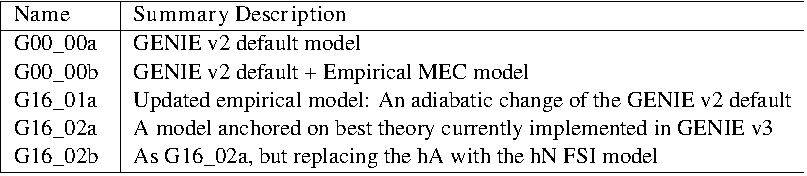
\includegraphics[width=\textwidth]{images/model_summaries.pdf}
    \caption{A brief overview the features which make up the individual model configurations in GENIE. These models will eventually all be tuned.}
    \label{tab:modelConfigs}
\end{figure}


Details on the first model to be tuned (G16\_01b) are as follows: 

\begin{itemize}
    \item Includes Empirical MEC
    \item CCQE process is Llewellyn-Smith Model
    \item Dipole Axial Form Factor - Depending on M\(_{A}\) = 0.99 GeV
    \item Nuclear model: Fermi Gas Model - Bodek, Ritchie
\end{itemize}

\begin{figure}[h!]
    \centering
    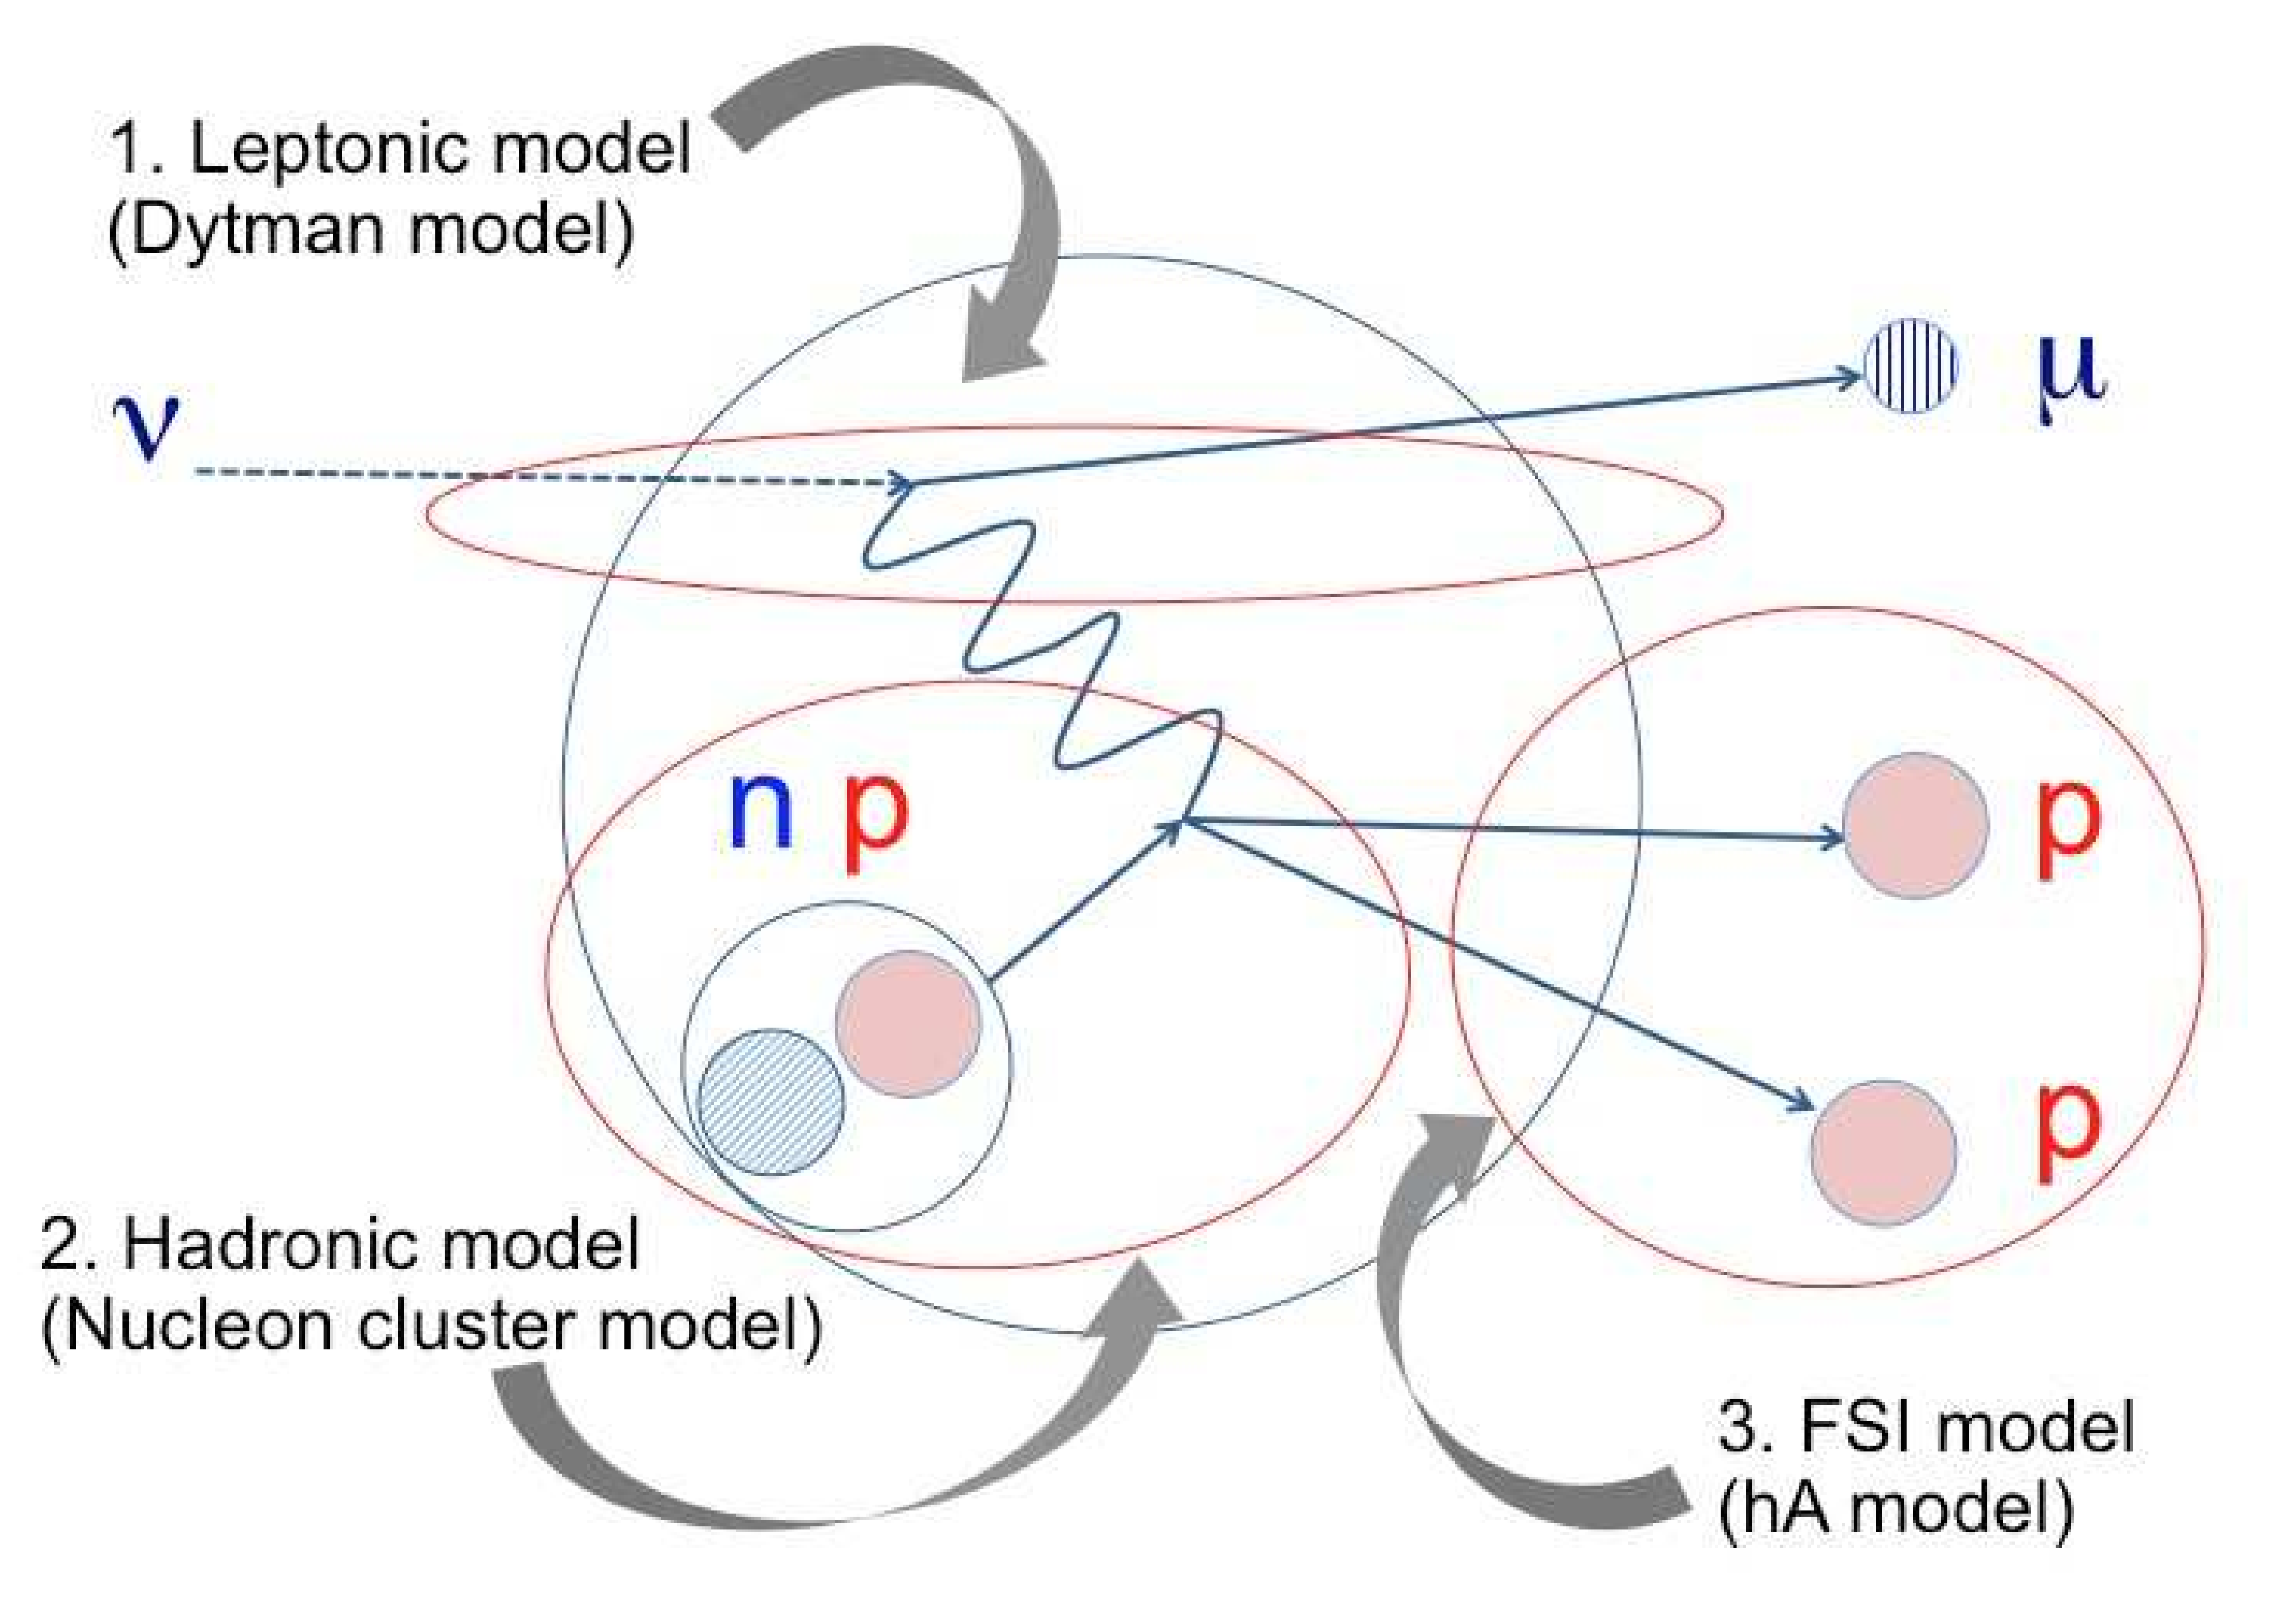
\includegraphics[width=.5\textwidth]{images/mec_model_genie.png}
    \caption{The models involved in the construction of the MEC model in neutrino event generation.}
    \label{fig:MECSchem}
\end{figure}

\clearpage

\begin{figure}[h!]
    \centering
    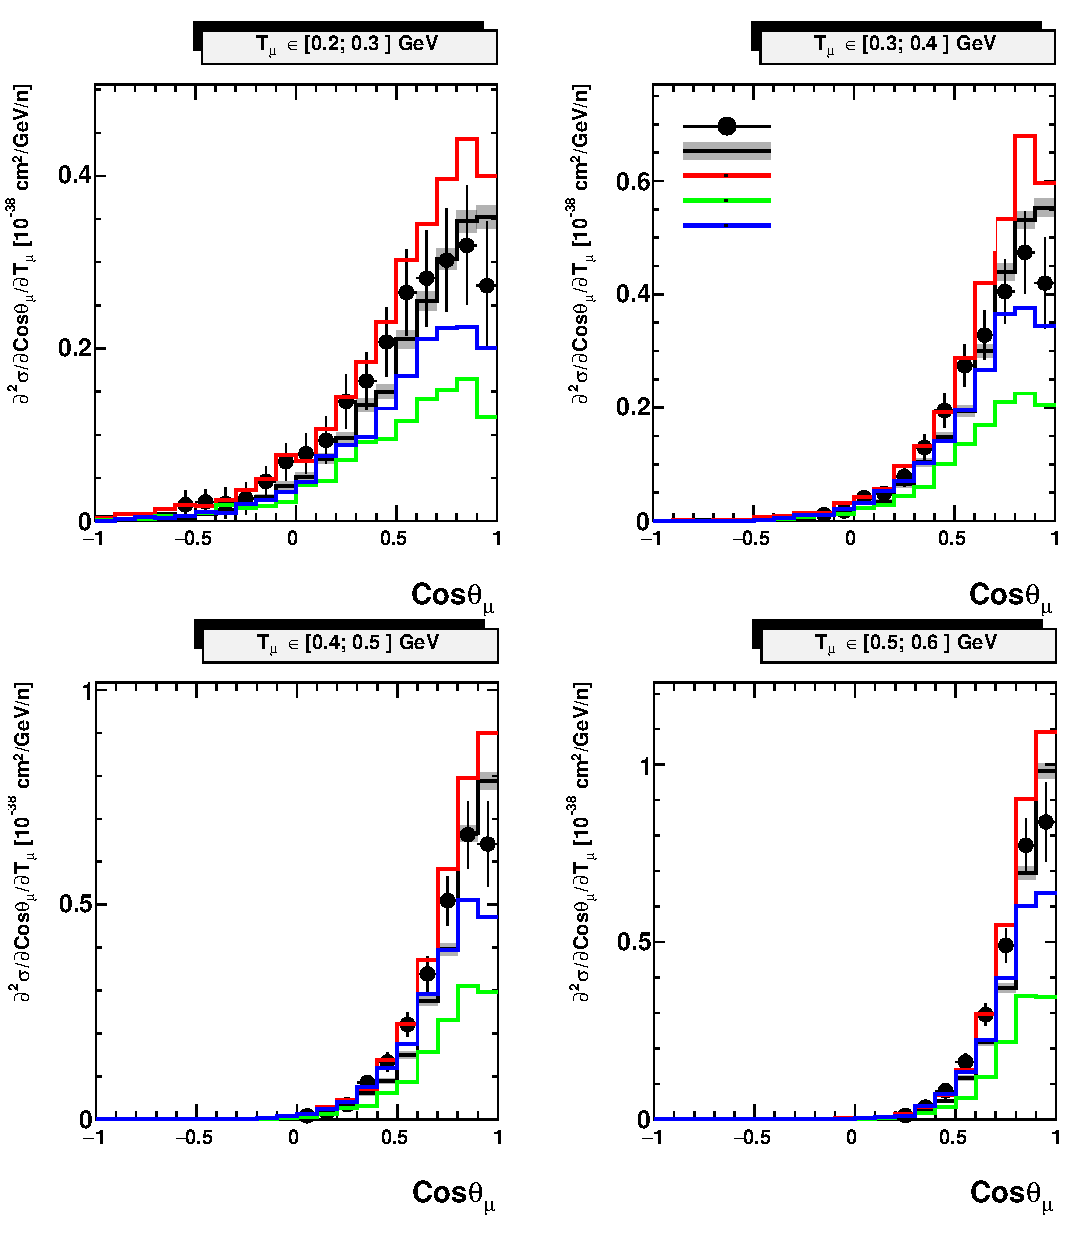
\includegraphics[width=\textwidth]{images/MB_Comp_numubar.pdf}
    \put(-120,450){\scriptsize MiniBooNE \(\bar{\nu}_{\mu}\)CCQE, 2013}
    \put(-120,440){\scriptsize G00\_00a}
    \put(-120,430){\scriptsize G00\_00b}
    \put(-120,420){\scriptsize G16\_01a}
    \put(-120,410){\scriptsize G16\_02b}
    \caption{An example comparison between 4 GENIE models (described briefly in Figure~\ref{tab:modelConfigs}) and MiniBooNE \(\bar{\nu}_{\mu}\)CCQE data from 2013. The models fit the data with varying accuracies. It can be seen that even the closest fitting model is does not perfectly predict the trend seen in the data, therefore tuning is needed to fully optimise these fits.}
    \label{fig:MBComp}
\end{figure}

\clearpage

This model takes the updated default GENIE model (G16\_01a) and additionally addresses the abnormalities seen in recent experiments by incorporating the MEC interaction, described schematically in terms of the theoretical models involved in Figure~\ref{fig:MECSchem} \cite{MEC}. 

Datasets currently involved in the fit come from MiniBooNE, T2K and Minerva. An example of a comparison between the MiniBooNE \(\bar{\nu}_{\mu}\) CCQE data set from 2013 and 4 different GENIE predictions is shown in Figure~\ref{fig:MBComp}.

Although the G16\_02b model is the most theoretically driven, it does not always provide the best fit to the data sets. For instance, in the MiniBooNE \(\nu\) CCQE data from 2010, the G16\_02b model fits better than both G00\_00a and G00\_00b, these fits are shown and quantified in Figure~\ref{fig:MBnu}. However, in the MiniBooNE \(\bar{\nu}\) CCQE data from 2013, Figure~\ref{fig:MBnubar} shows that the G00\_00b model had the best fit of the same three. Similarly in Figure~\ref{fig:T2Knu} which is the comparison between the same models for the T2K ND280 \(\nu\) CC0\(\pi\) data from 2015, the G00\_00a model fit best.

\clearpage

\begin{figure}[h!]
    \centering
    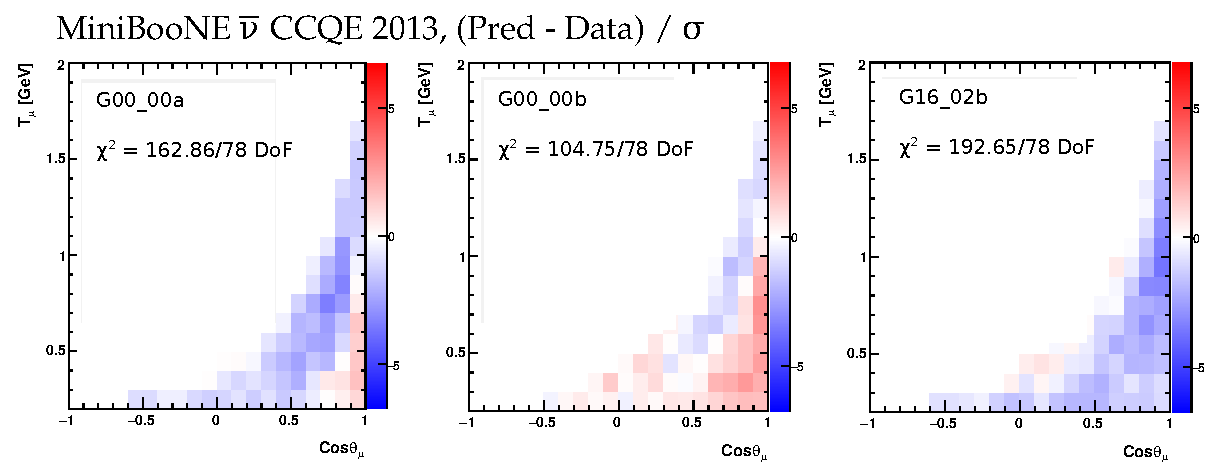
\includegraphics[width=\textwidth]{images/MB_numubar.pdf}
    \put(-183,156){ \( \partial ^2 \sigma / \partial \mbox{cos} \theta_{\mu} / \partial \mbox{T}_{\mu} \) [10\(^{-38}\)cm\(^{2}\)/GeV/n]}
    \caption{ A comparison between the MiniBooNE \(\bar{\nu}\) CCQE 2010 data set and 3 of the GENIE model configurations, left: G00\_00a, middle: G00\_00b, right: G16\_02b. Taking the best fit to be the distribution with the lowest \(\chi^2\) / DoF, the G00\_00b model predicts the dataset best.}
    \label{fig:MBnubar}
\end{figure}

\begin{figure}[h!]
    \centering
    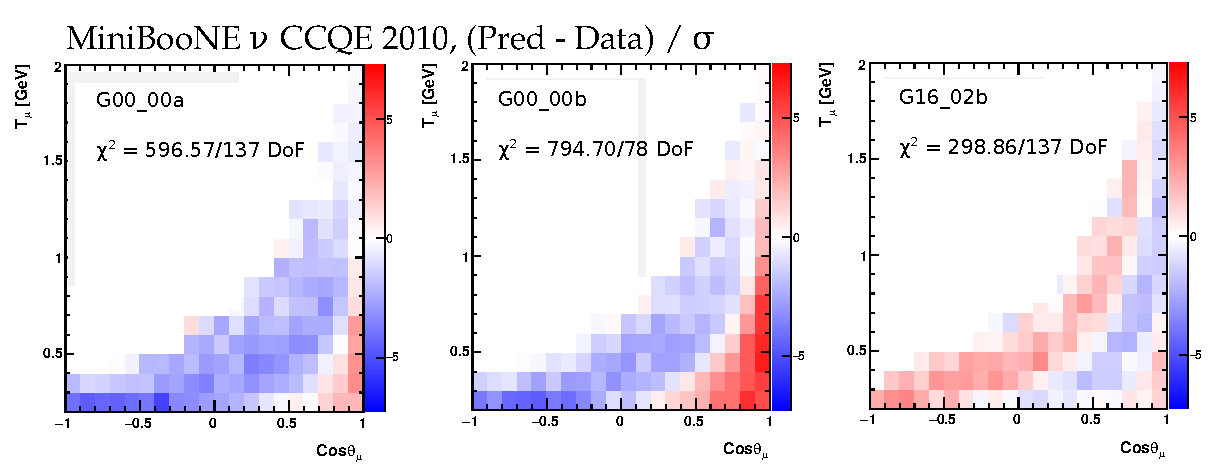
\includegraphics[width=\textwidth]{images/MB_numu.pdf}
    \put(-183,156){ \( \partial ^2 \sigma / \partial \mbox{cos} \theta_{\mu} / \partial \mbox{T}_{\mu} \) [10\(^{-38}\)cm\(^{2}\)/GeV/n]}
    \caption{ A comparison between the MiniBooNE \(\nu\) CCQE 2013 data set and the same GENIE model configurations as in Figure~\ref{fig:MBnu}. The same best fit definition means the G16\_02b model predicts the dataset best.}
    \label{fig:MBnu}
\end{figure}

\begin{figure}[h!]
    \centering
    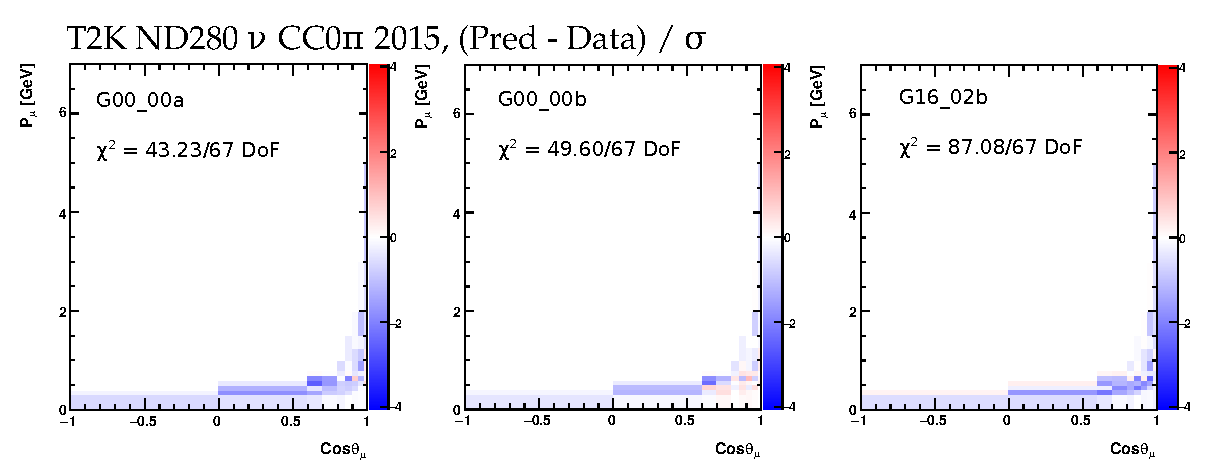
\includegraphics[width=\textwidth]{images/T2K_numu.pdf}
    \put(-183,156){ \( \partial ^2 \sigma / \partial \mbox{cos} \theta_{\mu} / \partial \mbox{P}_{\mu} \) [10\(^{-38}\)cm\(^{2}\)/GeV/n]}
    \caption{ A comparison between the T2K \(\nu\) CC0\(\pi\) 2015 data set and the same GENIE model configurations as in Figures~\ref{fig:MBnu} and~\ref{fig:MBnubar}. The same best fit definition means the G00\_00a model predicts the dataset best.}
    \label{fig:T2Knu}
\end{figure}

%\clearpage

Clearly, there are tensions between the datasets and no single theory best predicts all data. This tension will be a focal point when analysing the tuning results. 


\subsection{Professor}

The Professor software framework parameterises the Monte Carlo event generator's response to parameter shifts on a bin-by-bin basis \cite{prof}. The tuning is done through fitting parameters within models to data and has the ability to incorporate multiple parameters within models as well as fitting together multiple data sets. Professor therefore provides the opportunity to perform global tunings of theoretical models based on the extensive archive of neutrino scattering data which is publically available.

The tuning is done in a subset of parameter space rather than on the full Monte Carlo, this space is defined by the x-axis in Figure~\ref{fig:profSchem} which is a schematic diagram of the fitting process. Only parameterising a sample of the Monte Carlo drastically reduces the computational expense of the process. The tuning is perfomed on multiple parameters in one go, and the nominal value for each is calculated using a \(\chi^2\) minimisation \cite{prof}. 

\begin{figure}[h!]
    \centering
    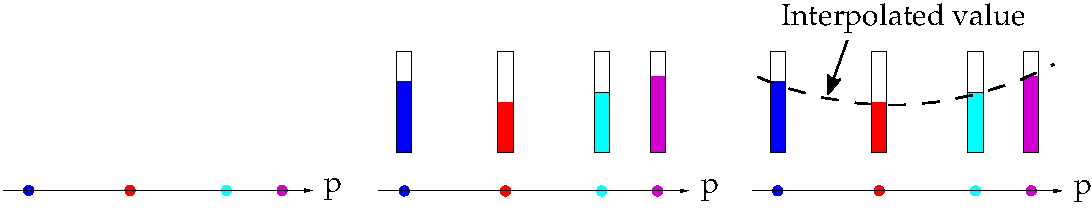
\includegraphics[width=\textwidth]{images/prof_schem.pdf}
    \caption{A schematic of the Professor tuning method. Left: the parameter space is selected. Middle: The behaviour of each parameter in an individual bin is observed. Right: A parameter-dependent interpolation is constructed \( I(p) \) from the whole parameter space. The process is repeated for every bin. }
    \label{fig:profSchem}
\end{figure}

\subsection{Results}

To date, the fit has been performed on 6 parameters within the G16\_01b model, the results of which are given in Figure~\ref{fig:paramRes} alongside the nominal - most physical - value for each. 

\begin{figure}[h!]
    \centering
    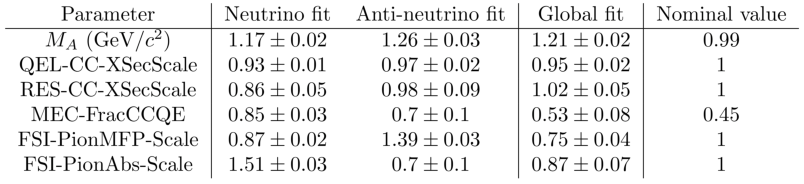
\includegraphics[width=\textwidth]{images/param_fit_results.pdf}
    \caption{Parameter fit results.}
    \label{fig:paramRes}
\end{figure}

Towards the global fit, the G16\_01b model was also tuned separetely to 5 sets of data: MiniBooNE CCQE \(\nu_{\mu}\), MiniBooNE CCQE \(\bar{\nu}_{\mu}\), Minerva CCQE \(\nu_{\mu}\), Mineva CCQE \(\bar{\nu}_{\mu}\) and T2K CC 0\(\pi\). The results of the individual and global fits are given in Figure~\ref{fig:exRes} 

\begin{figure}[h!]
    \centering
    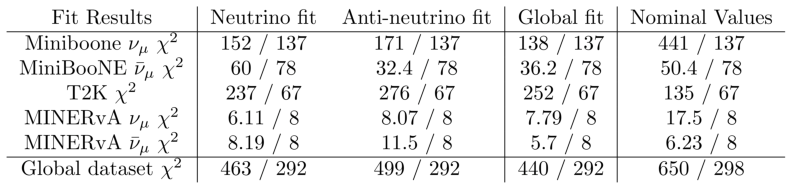
\includegraphics[width=\textwidth]{images/exp_fit_results.pdf}
    \caption{Experiment fit results.}
    \label{fig:exRes}
\end{figure}

Graphical slices of the experimental results for MiniBooNE \(\nu_{\mu}\), Minerva \(\nu_{\mu}\) and T2K are shown in Figure~\ref{fig:globRes} in order to visually demonstrate the comparison between the model before and after tuning on each data set.  

\begin{figure}[h!]
    \begin{picture}(436,436)
        \centering
        \includegraphics[width=\textwidth]{images/fit_results.pdf}
        \put(-415,275){\rotatebox{90}{\small \( \partial^{2} \sigma \)/\( \partial \)T\(_{\mu}\)/\( \partial \)cos\(\theta_{\mu}\) [10\(^{-38}\) cm\(^{2}\)/GeV/n] }}
        \put(-210,306){\rotatebox{90}{\small d\(\sigma\)/dQ\(^{2}\) [10\(^{-38}\) cm\(^{2}\)/GeV\(^{2}\)/n] }}
        \put(-350,105){\rotatebox{90}{\small \(\partial^{2} \sigma \)/\(\partial\)P\(_{\mu}\)/\(\partial\) cos\(\theta_{\mu}\) }}
        \put(-335,95){\rotatebox{90}{\small [10\(^{-38}\) cm\(^{2}\)/GeV/n] }}
        \put(-280,240){ T\(_{\mu}\) [GeV]}
        \put(-60,240){ Q\(^{2}\) [GeV\(^{2}\)]}
        \put(-150,45){ P\(_{\mu}\) [GeV]}
    \end{picture}
    \caption{Global fit results.}
    \label{fig:globRes}
\end{figure}

\clearpage
